% ═══════════════════════════════════════════════════════════════
%  Research Group Presentation — 14 April 2026
%  ADoTA: Angle-Dependent Dose Transformer Algorithm
%  Current Results, Limitations, and the Case for Active Learning
%  Author: Mikołaj Stryja
% ═══════════════════════════════════════════════════════════════
\documentclass[aspectratio=169, 10pt]{beamer}

% ── Theme & colours ─────────────────────────────────────────
\usetheme{Madrid}
\usecolortheme{default}
\definecolor{tudelft}{RGB}{0,100,172}
\setbeamercolor{structure}{fg=tudelft}
\setbeamercolor{title}{fg=white,bg=tudelft}
\setbeamercolor{frametitle}{fg=white,bg=tudelft}
\setbeamertemplate{navigation symbols}{}
\setbeamertemplate{footline}{%
  \leavevmode\hbox{%
    \begin{beamercolorbox}[wd=.33\paperwidth,ht=2.5ex,dp=1ex,center]{author in head/foot}%
      \usebeamerfont{author in head/foot}\insertshortauthor
    \end{beamercolorbox}%
    \begin{beamercolorbox}[wd=.34\paperwidth,ht=2.5ex,dp=1ex,center]{title in head/foot}%
      \usebeamerfont{title in head/foot}\insertshorttitle
    \end{beamercolorbox}%
    \begin{beamercolorbox}[wd=.33\paperwidth,ht=2.5ex,dp=1ex,right]{date in head/foot}%
      \usebeamerfont{date in head/foot}\insertframenumber{}/\inserttotalframenumber\hspace*{2ex}
    \end{beamercolorbox}}%
  \vskip0pt%
}

% ── Packages ────────────────────────────────────────────────
\usepackage{graphicx}
\usepackage{booktabs}
\usepackage{amsmath,amssymb}
\usepackage{siunitx}
\usepackage{tikz}
\usetikzlibrary{arrows.meta,positioning,calc,shapes.geometric,decorations.pathreplacing}
\usepackage{xcolor}
\usepackage{multirow}
\usepackage[normalem]{ulem}  % for \sout (strikethrough)

% ── Meta ────────────────────────────────────────────────────
\title[ADoTA]{ADoTA: Angle-Dependent Dose Transformer Algorithm\\[4pt]
{\small Deep Learning Proton Dose Engine —\\Current Results, Limitations, and the Case for Active Learning}}
\author[M.~Stryja]{Mikołaj Stryja}
\institute{Department of Radiation Science \& Technology, TU Delft}
\date{14 April 2026}

% ════════════════════════════════════════════════════════════
\begin{document}

% ── Title ───────────────────────────────────────────────────
\begin{frame}[plain]
  \titlepage
\end{frame}

% ── Outline ─────────────────────────────────────────────────
\begin{frame}{Outline}
  \tableofcontents
\end{frame}

% ════════════════════════════════════════════════════════════════
\section{The Problem: Proton Dose Calculation}
% ════════════════════════════════════════════════════════════════

\begin{frame}{Why Dose Calculation Matters}
  \begin{columns}[T]
    \begin{column}{0.55\textwidth}
      \begin{itemize}\setlength{\itemsep}{4pt}
        \item Pencil Beam Scanning Proton Therapy (PBSPT) delivers dose
              via thousands of narrow proton beamlets, each modulated in
              \textbf{energy} and \textbf{direction}.
        \item The treatment plan is constructed from the \textbf{dose
              influence matrix} $d_{ij}$: dose deposited in voxel~$i$ by
              beamlet~$j$.
        \item Accurate 3D dose calculation is critical because of:
        \begin{itemize}
          \item steep dose gradients (Bragg peak),
          \item range sensitivity to tissue heterogeneity,
          \item setup and range uncertainties.
        \end{itemize}
      \end{itemize}
    \end{column}
    \begin{column}{0.42\textwidth}
      \begin{block}{Clinical context}
        \begin{itemize}\setlength{\itemsep}{2pt}
          \item \textbf{Robust planning} — requires many uncertainty
                scenarios $\Rightarrow$ many $d_{ij}$ recomputations.
          \item \textbf{Online adaptive therapy} — dose must be
                recalculated in seconds, not hours.
          \item \textbf{Plan optimisation} — iterative solver calls
                the dose engine thousands of times.
        \end{itemize}
      \end{block}
    \end{column}
  \end{columns}
\end{frame}

\begin{frame}{Current Dose Engines and Their Limitations}
  \begin{table}
    \centering\small
    \begin{tabular}{lccl}
      \toprule
      \textbf{Method} & \textbf{Speed} & \textbf{Accuracy} & \textbf{Key limitation} \\
      \midrule
      Monte Carlo (MC) & \SI{43.6}{s}/beamlet & Gold standard &
        Computationally prohibitive \\
      Pencil Beam Alg.\ (PBA) & $\sim$\SI{0.7}{s}/beamlet & Moderate &
        Degrades in heterogeneous media \\
      GPU MC & $\sim$seconds & High &
        Still too slow for online adaptive \\
      \bottomrule
    \end{tabular}
  \end{table}

  \vspace{6pt}
  \begin{block}{The gap}
    We need a dose engine that is simultaneously:
    \begin{enumerate}
      \item \textbf{Fast}: sub-second per beamlet (ideally ms-scale),
      \item \textbf{Accurate}: MC level fidelity (GPR $>$ \SI{98}{\percent}),
      \item \textbf{General}: arbitrary beam energies, angles, and anatomies.
    \end{enumerate}
  \end{block}
\end{frame}

\begin{frame}{Deep Learning Approaches to Proton Dose Calculation}
  \begin{columns}[T]
    \begin{column}{0.48\textwidth}
      \textbf{Prior work:}
      \begin{itemize}\setlength{\itemsep}{3pt}
        \item \textbf{DoTA} (Pastor-Serrano \& Perkó, 2022):\\
              Transformer + U-Net, multi-energy,\\
              \SI{5}{ms}/beamlet.
        \item \textbf{CC-LSTM} (Neishabouri et al., 2025):\\
              Convolutional LSTM, 98\% fewer parameters,
              mono-energetic.
        \item \textbf{MED-LSTM} (Pang et al., 2025):\\
              Multi-energy LSTM, high GPR on limited energy range.
      \end{itemize}
    \end{column}
    \begin{column}{0.48\textwidth}
      \textbf{Shared bottleneck:}

      \vspace{4pt}
      All prior methods require the CT volume to be
      \textbf{rotated and reinterpolated} so the voxel grid is
      \emph{perpendicular} to each beamlet direction
      (Beam's Eye View).

      \vspace{6pt}
      \begin{alertblock}{Preprocessing overhead}
        Grid reinterpolation $\approx$ \textbf{\SI{1.3}{s}/beamlet}
        — three orders of magnitude slower than the neural network
        inference itself ($\sim$\SI{2}{ms}).
      \end{alertblock}

      \vspace{4pt}
      {\small For a plan with 5\,000 beamlets, this amounts to
       $\sim$1.8\,hours of preprocessing alone.}
    \end{column}
  \end{columns}
\end{frame}

% ════════════════════════════════════════════════════════════════
\section{ADoTA: Our Approach}
% ════════════════════════════════════════════════════════════════

\begin{frame}{Key Idea: Eliminate Per-Beamlet Reinterpolation}
  \vspace{-4pt}
  \begin{columns}[T]
    % ── LEFT: Prior pipeline ──────────────────────────────
    \begin{column}{0.46\textwidth}
      \begin{center}
        {\small\textbf{Prior methods} (DoTA, CC-LSTM, MED-LSTM)}

        \vspace{2pt}
        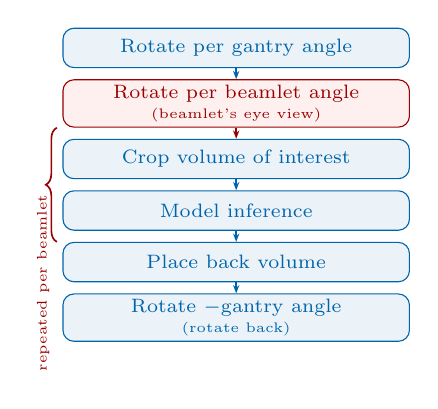
\begin{tikzpicture}[
          box/.style={draw=tudelft, rounded corners=4pt,
                      minimum width=4.4cm, minimum height=0.5cm,
                      font=\scriptsize, text=tudelft, fill=tudelft!8,
                      align=center, inner sep=2pt},
          slow/.style={draw=red!60!black, rounded corners=4pt,
                      minimum width=4.4cm, minimum height=0.5cm,
                      font=\scriptsize, text=red!60!black, fill=red!6,
                      align=center, inner sep=2pt},
          arr/.style={-{Stealth[length=3pt]}, semithick, tudelft},
          redarr/.style={-{Stealth[length=3pt]}, semithick, red!60!black},
          brace/.style={decorate, decoration={brace, amplitude=4pt,
                        mirror, raise=2pt}, semithick, red!60!black}
        ]
          \node[box]  (g1)  {Rotate per gantry angle};
          \node[slow, below=4pt of g1]  (bev) {Rotate per beamlet angle\\[-1pt]{\tiny(beamlet's eye view)}};
          \node[box, below=4pt of bev]  (crop1) {Crop volume of interest};
          \node[box, below=4pt of crop1] (inf1) {Model inference};
          \node[box, below=4pt of inf1] (place1) {Place back volume};
          \node[box, below=4pt of place1] (rot1) {Rotate $-$gantry angle\\[-1pt]{\tiny(rotate back)}};
          \draw[arr]    (g1) -- (bev);
          \draw[redarr] (bev) -- (crop1);
          \draw[arr]    (crop1) -- (inf1);
          \draw[arr]    (inf1) -- (place1);
          \draw[arr]    (place1) -- (rot1);
          % brace marking the per-beamlet block
          \draw[brace] (bev.south west) -- (place1.north west)
            node[midway, left=7pt, font=\tiny, text=red!60!black,
                 align=center, rotate=90] {repeated per beamlet};
        \end{tikzpicture}

        \vspace{2pt}
        {\scriptsize\color{red!60!black}
         Reinterpolation \textbf{per beamlet}:
         $\sim$\SI{1.3}{s} overhead each}
      \end{center}
    \end{column}
    % ── RIGHT: ADoTA pipeline ─────────────────────────────
    \begin{column}{0.46\textwidth}
      \begin{center}
        {\small\textbf{ADoTA} (this work)}

        \vspace{2pt}
        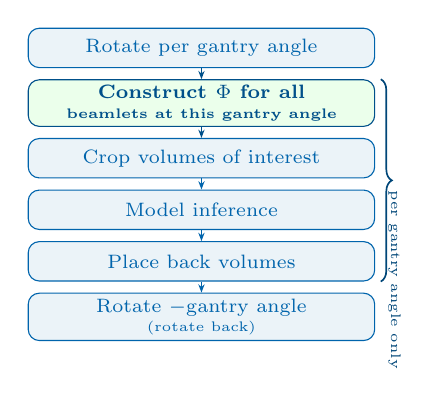
\begin{tikzpicture}[
          box/.style={draw=tudelft, rounded corners=4pt,
                      minimum width=4.4cm, minimum height=0.5cm,
                      font=\scriptsize, text=tudelft, fill=tudelft!8,
                      align=center, inner sep=2pt},
          new/.style={draw=tudelft!80!black, rounded corners=4pt,
                      minimum width=4.4cm, minimum height=0.5cm,
                      font=\scriptsize\bfseries, text=tudelft!80!black,
                      fill=green!8, align=center, inner sep=2pt},
          arr/.style={-{Stealth[length=3pt]}, semithick, tudelft},
          newarr/.style={-{Stealth[length=3pt]}, semithick, tudelft!80!black},
          brace/.style={decorate, decoration={brace, amplitude=4pt,
                        raise=2pt}, semithick, tudelft!70!black}
        ]
          \node[box] (g2) {Rotate per gantry angle};
          \node[new, below=4pt of g2] (phi) {Construct $\Phi$ for all\\[-1pt]{\tiny beamlets at this gantry angle}};
          \node[box, below=4pt of phi] (crop2) {Crop volumes of interest};
          \node[box, below=4pt of crop2] (inf2) {Model inference};
          \node[box, below=4pt of inf2] (place2) {Place back volumes};
          \node[box, below=4pt of place2] (rot2) {Rotate $-$gantry angle\\[-1pt]{\tiny(rotate back)}};
          \draw[newarr] (g2) -- (phi);
          \draw[newarr] (phi) -- (crop2);
          \draw[arr]    (crop2) -- (inf2);
          \draw[arr]    (inf2) -- (place2);
          \draw[arr]    (place2) -- (rot2);
          % brace marking the per-gantry block
          \draw[brace] (phi.north east) -- (place2.south east)
            node[midway, right=7pt, font=\tiny, text=tudelft!70!black,
                 align=center, rotate=-90] {per gantry angle only};
        \end{tikzpicture}

        \vspace{2pt}
        {\scriptsize\color{tudelft!80!black}
         $\Phi$ computed \textbf{analytically} (no grid rotation):
         $\sim$\SI{0.2}{s}/beamlet}
      \end{center}
    \end{column}
  \end{columns}

  \vspace{4pt}
  \centering
  \begin{beamercolorbox}[wd=0.88\textwidth, rounded=true, shadow=true,
    sep=3pt]{block body}
    \centering\small
    \textbf{Novelty:} Replace the expensive per-beamlet grid
    reinterpolation with a fast analytical beamlet shape projection
    $\Phi$ $\Rightarrow$ \textbf{6.5$\times$ end-to-end speedup}
    while maintaining MC-level accuracy.
  \end{beamercolorbox}
\end{frame}

\begin{frame}{The Beamlet Shape Projection $\Phi$}
  For a beamlet with deflection angles $\theta_x, \theta_y$ and
  energy-dependent spot sizes $\sigma_x(\epsilon), \sigma_y(\epsilon)$
  from the Beam Data Library:

  \vspace{4pt}
  \textbf{Step 1 — Transform to beam-aligned coordinates:}
  \[
    \mathbf{u}' = R_y(\theta_x)\, R_x(\theta_y)\,
    (\mathbf{u} - \mathbf{u}_0)
  \]
  where $\mathbf{u}_0$ is the beamlet entrance point on the CT grid.

  \vspace{4pt}
  \textbf{Step 2 — Evaluate Gaussian flux at every voxel:}
  \[
    \Phi(\mathbf{u}) = \frac{1}{2\pi\,\sigma_x(\epsilon)\,\sigma_y(\epsilon)}
    \exp\!\left(
      -\frac{(x')^2}{2\sigma_x(\epsilon)^2}
      -\frac{(y')^2}{2\sigma_y(\epsilon)^2}
    \right)
  \]

  \vspace{4pt}
  \begin{block}{Why this works}
    $\Phi$ encodes the beam \emph{direction} and \emph{lateral profile}
    explicitly.  The network sees $[\text{CT} \mid \Phi]$ as a
    two-channel 3D input — no grid realignment per beamlet is needed.
  \end{block}
\end{frame}

\begin{frame}{Network Architecture}
  \vspace{-4pt}
  \begin{columns}[T]
    \begin{column}{0.38\textwidth}
      {\small\textbf{ADoTA = 3D U-Net + Transformer}}

      \vspace{3pt}
      {\scriptsize
      \begin{itemize}\setlength{\itemsep}{2pt}
        \item[\textbullet] \textbf{Two inputs}: a 3D CT patch with
              the beamlet shape projection $\Phi$, plus beam
              energy~$\epsilon$.
        \item[\textbullet] \textbf{Encoder} compresses the volume
              through 4 stages of convolutions, extracting
              increasingly abstract features.
        \item[\textbullet] \textbf{Transformer bottleneck} captures
              long-range dependencies along the beam depth —
              key for modelling the Bragg peak build-up.
        \item[\textbullet] \textbf{Decoder} reconstructs the 3D
              dose, guided by skip connections that preserve
              spatial detail from the encoder.
        \item[\textbullet] \textbf{Output}: predicted dose $\hat{D}$
              on the same grid as the input CT.
      \end{itemize}
      }
    \end{column}
    \begin{column}{0.59\textwidth}
      \vspace{-6pt}
      \begin{center}
        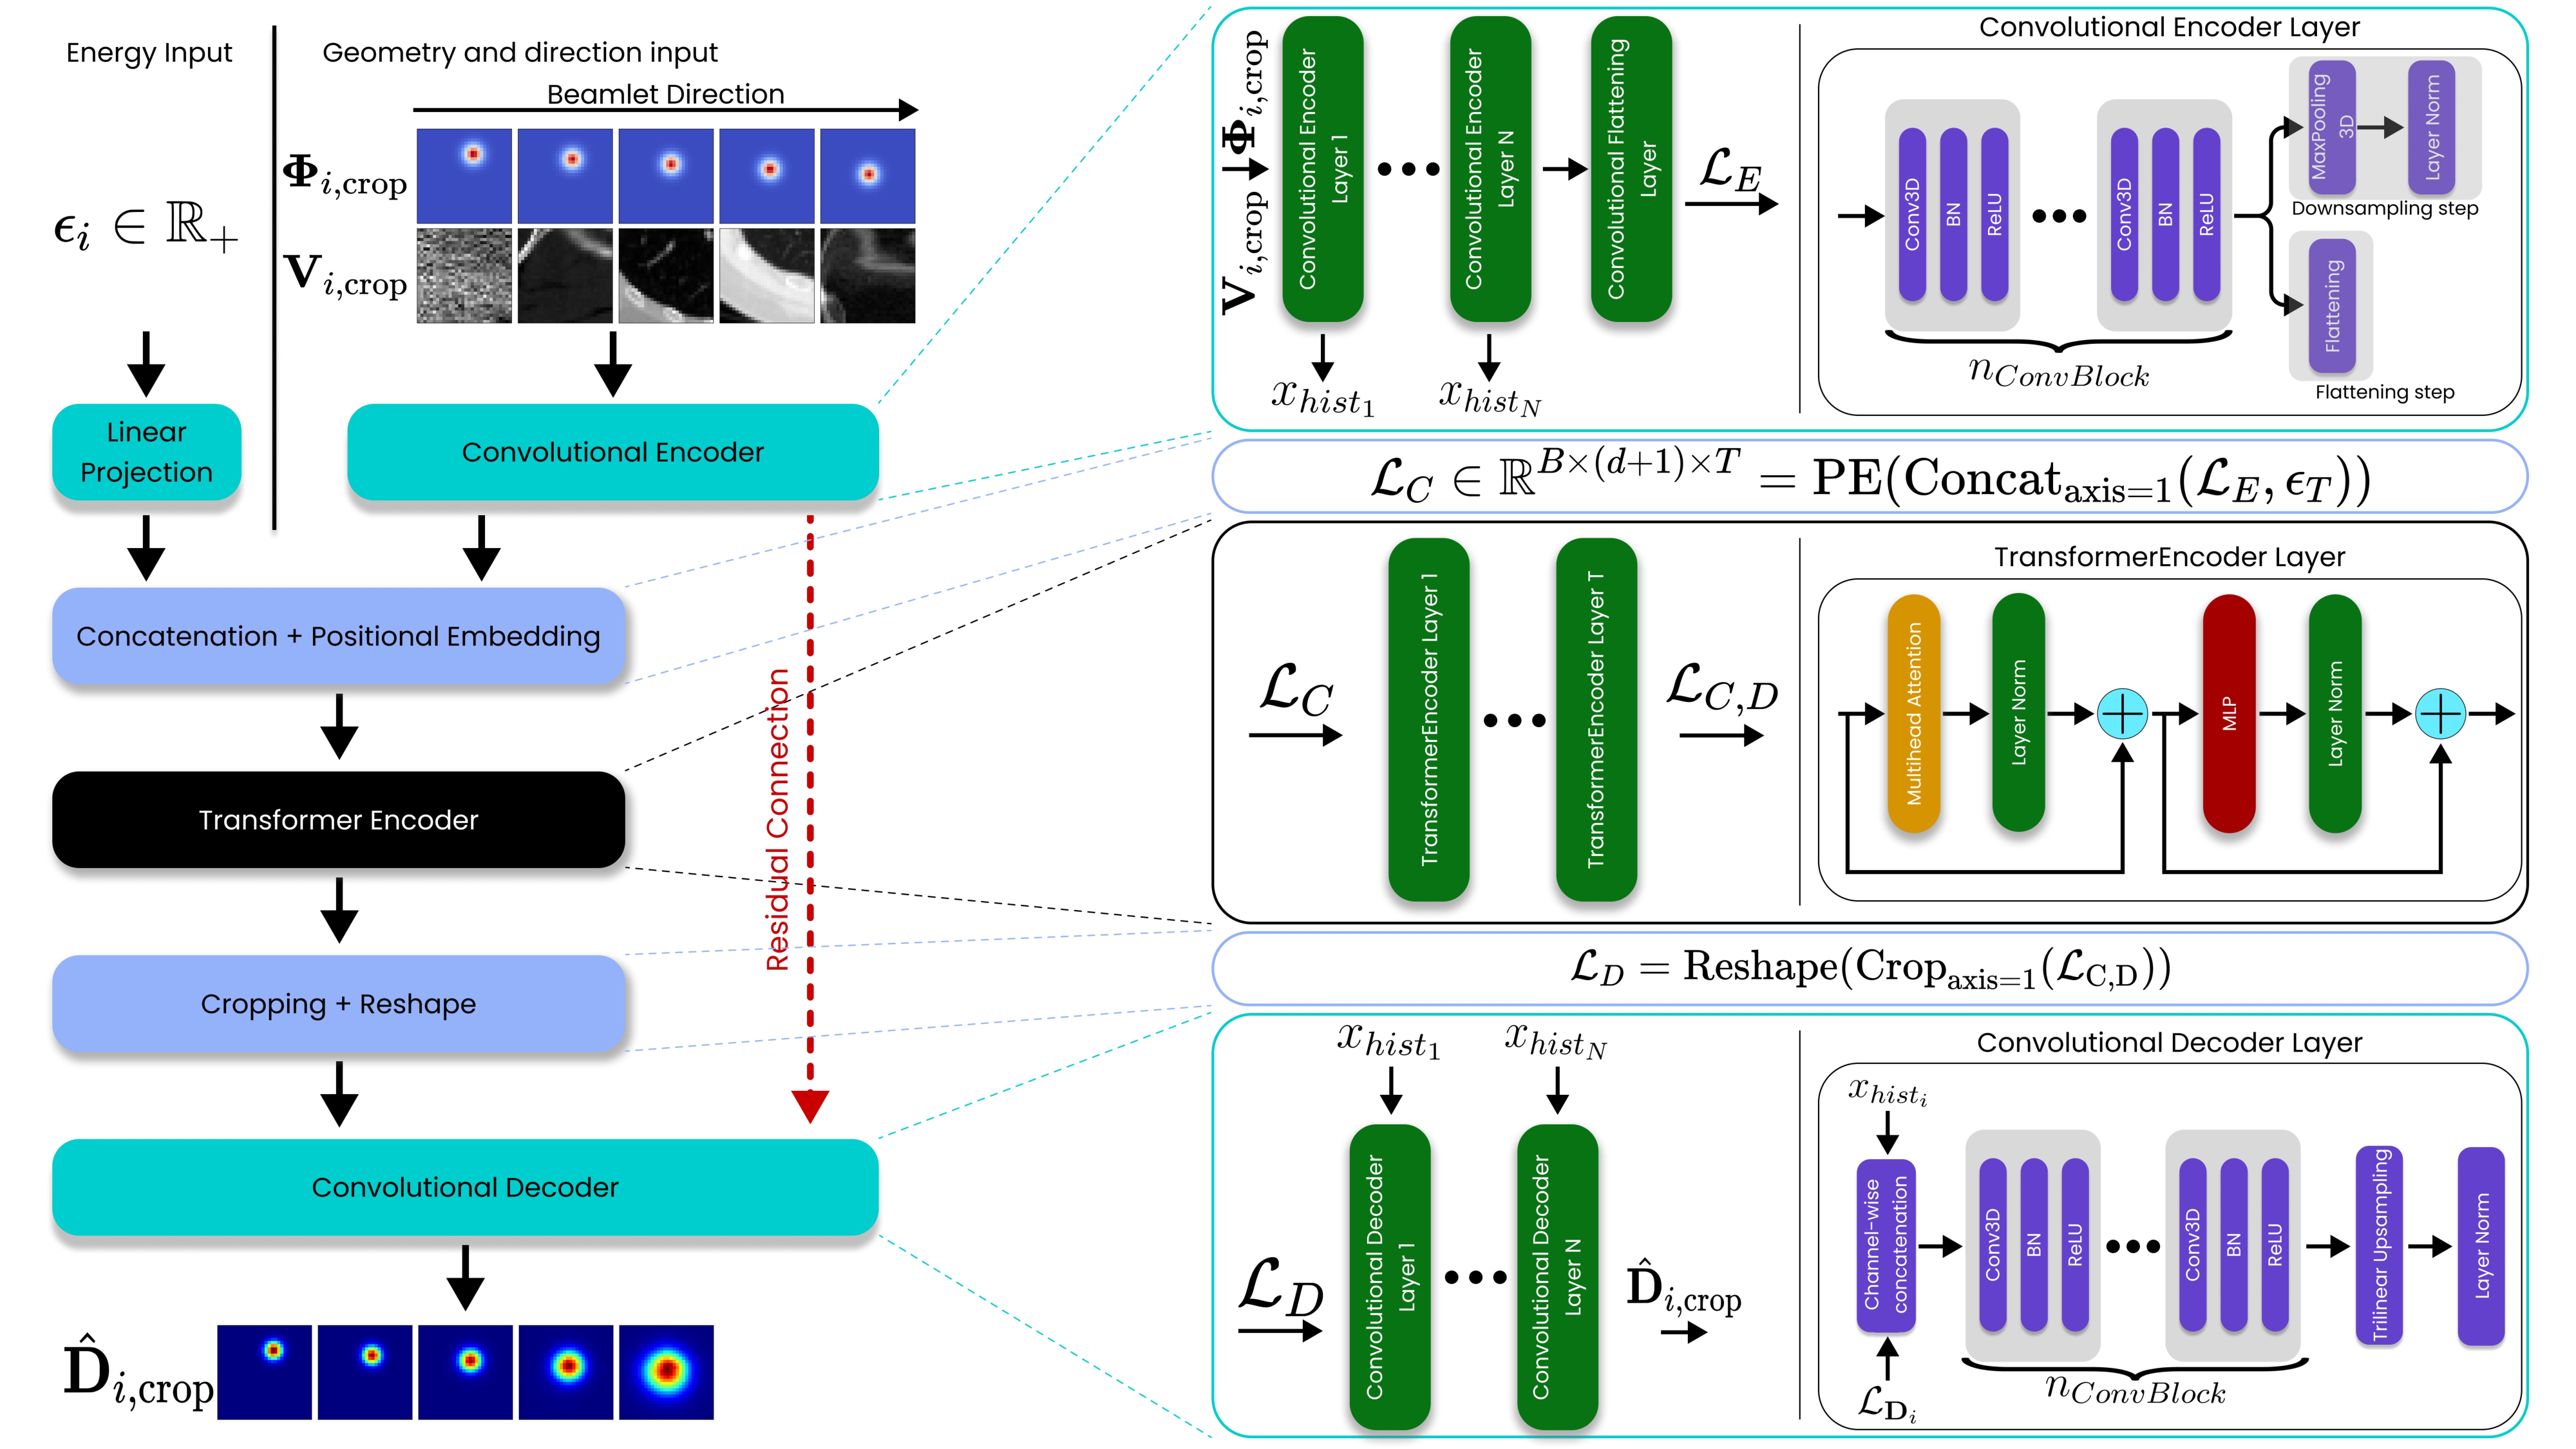
\includegraphics[width=\linewidth,height=0.82\textheight,keepaspectratio]{figures/ModelArchitectureFull_final.pdf}
      \end{center}
    \end{column}
  \end{columns}
\end{frame}

\begin{frame}{Data Generation: Ensuring Angular and Energy Variability}
  \vspace{-6pt}
  \begin{columns}[T]
    % ── LEFT: Step 1 ──────────────────────────────────────
    \begin{column}{0.48\textwidth}
      \begin{center}
        {\small\textbf{Step 1 — Sample a beamlet direction}}

        \vspace{1pt}
        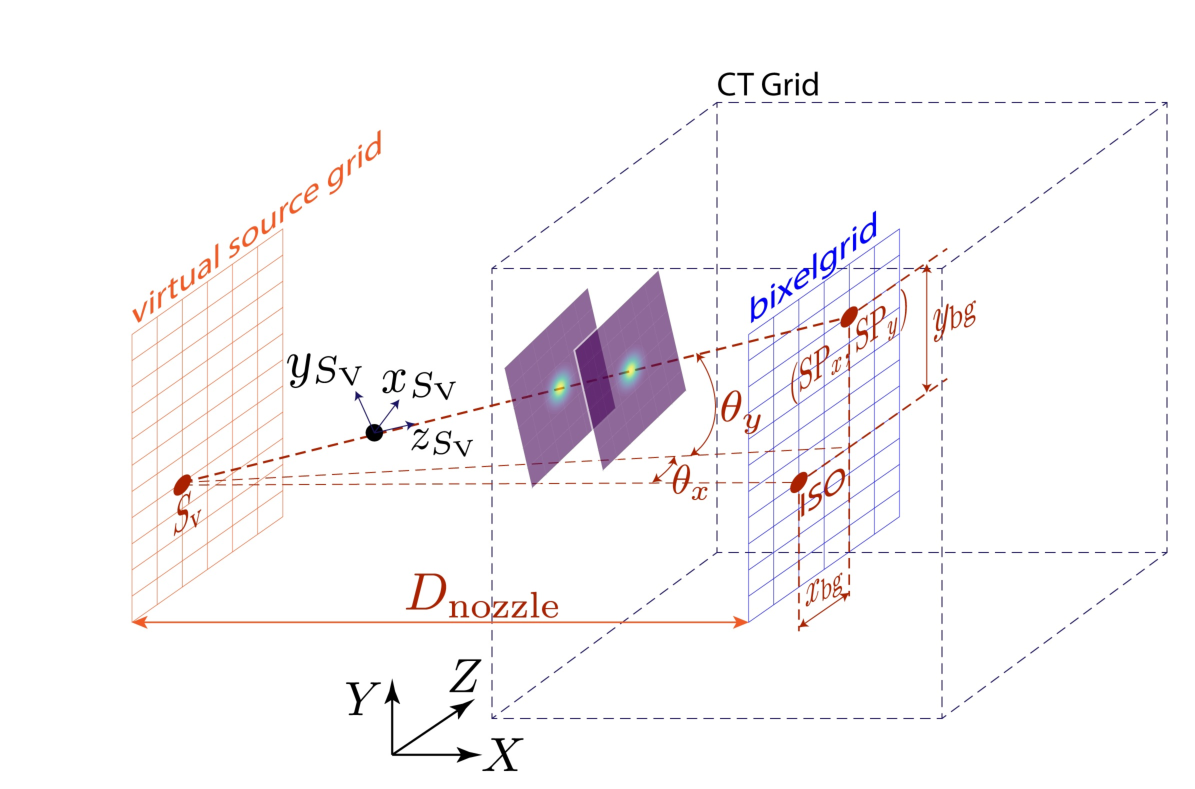
\includegraphics[width=0.78\linewidth]{figures/FirstSamplingPoint_v2.pdf}

        \vspace{1pt}
        {\scriptsize A spot position $(\text{SP}_x, \text{SP}_y)$ is
         sampled on the isocenter plane such that
         $|\theta_{x,y}| < 2.5^{\circ}$ w.r.t.\ the virtual
         source~$S_\text{v}$.  The beamlet shape $\Phi$ is
         a 2D Gaussian propagated along $z_{S_\text{v}}$.}
      \end{center}
    \end{column}
    % ── RIGHT: Step 2 ─────────────────────────────────────
    \begin{column}{0.48\textwidth}
      \begin{center}
        {\small\textbf{Step 2 — Translate the virtual source}}

        \vspace{1pt}
        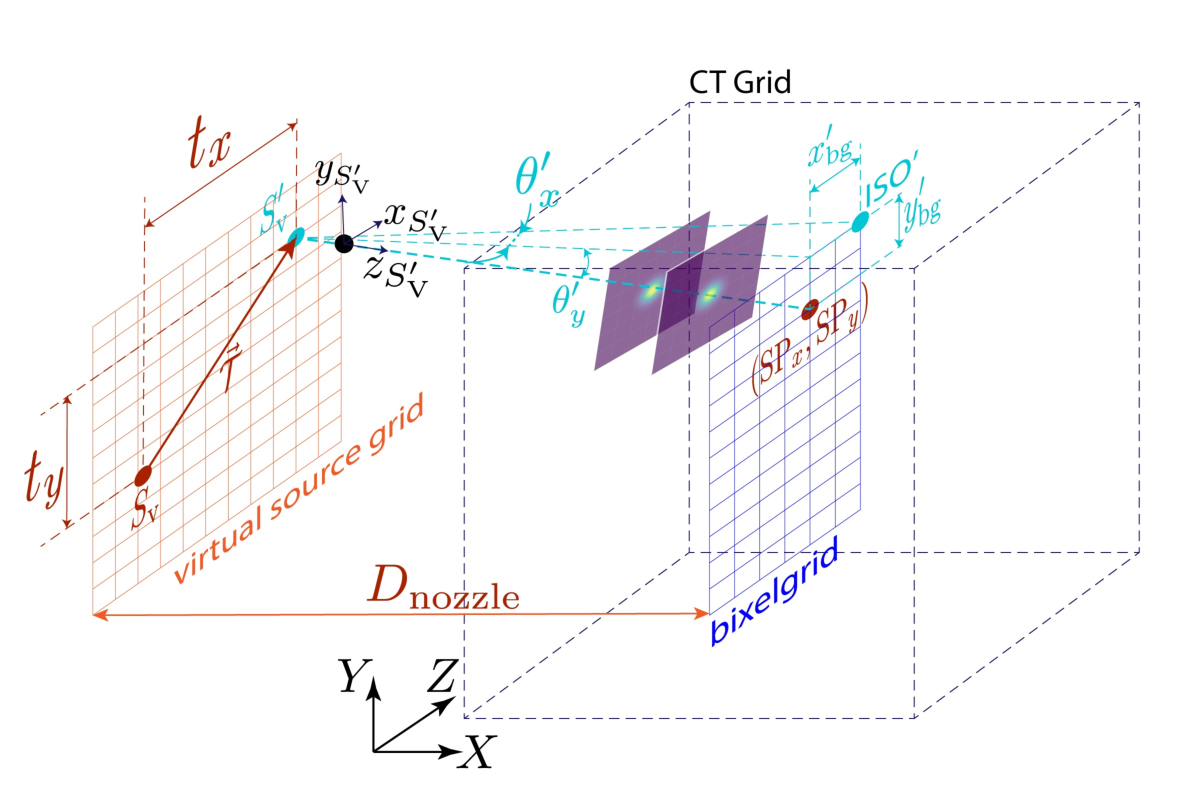
\includegraphics[width=0.78\linewidth]{figures/SecondSamplingPoint_v2.pdf}

        \vspace{1pt}
        {\scriptsize $S_\text{v}$ is shifted by
         $\vec{\mathcal{T}} = [t_x, t_y]$,
         $t_{x,y} \sim \mathcal{U}(-40, 40)$\,mm.
         Keeping the same spot, a new ray from
         $S'_\text{v}$ yields modified angles
         $(\theta'_x, \theta'_y)$ and a new $\Phi$
         along $z_{S'_\text{v}}$.}
      \end{center}
    \end{column}
  \end{columns}

  \vspace{3pt}
  \begin{beamercolorbox}[wd=\textwidth, rounded=true, shadow=true,
    sep=3pt]{block body}
    \centering\scriptsize
    For each spot position: \textbf{2 virtual source positions}
    (nominal + translated) $\times$ \textbf{2 proton energies}
    $\Rightarrow$ the dataset covers both
    \textbf{angular variability} (beam direction) and
    \textbf{energy variability} (penetration depth / Bragg peak
    position).
  \end{beamercolorbox}
\end{frame}

\begin{frame}{Training Setup}
  \begin{columns}[T]
    \begin{column}{0.48\textwidth}
      \textbf{Data:}
      \begin{itemize}\setlength{\itemsep}{3pt}
        \item 108 CT scans (92 thoracic, 16 abdominal/pelvic)
              from public TCIA collections.
        \item 70\,285 unique training records, patient-level split.
        \item Each record: CT crop $V$, beamlet projection $\Phi$,
              energy $\epsilon$, MC dose $D$ ($10^7$ protons/beamlet).
        \item Grid: $160 \times 30 \times 30$ voxels at \SI{2}{mm}
              isotropic (320 $\times$ 60 $\times$ 60 mm).
        \item Data augmentation: random lateral crop + in-plane
              rotation $\Rightarrow$ $\sim$100$\times$ expansion.
      \end{itemize}
    \end{column}
    \begin{column}{0.48\textwidth}
      \textbf{Loss function:}
      \[
        \mathcal{L} = \alpha\, \mathcal{L}_{\text{MSE}}
        + (1-\alpha)\, \mathcal{L}_{\text{IDD}}
      \]
      \begin{itemize}\setlength{\itemsep}{3pt}
        \item $\mathcal{L}_{\text{MSE}}$: normalised voxel-wise MSE
              for spatial fidelity.
        \item $\mathcal{L}_{\text{IDD}}$: integral depth dose profile
              loss to enforce correct Bragg peak range.
        \item $\alpha = 0.7$ (grid search).
      \end{itemize}

      \vspace{4pt}
      \textbf{Optimiser:} AdamW, $\text{lr} = 10^{-3}$,
      ReduceLROnPlateau, early stopping (100 epochs).

      \vspace{4pt}
      \textbf{Hardware:} NVIDIA A40 GPU, batch size 56.
    \end{column}
  \end{columns}
\end{frame}

% ════════════════════════════════════════════════════════════════
\section{Results}
% ════════════════════════════════════════════════════════════════

\begin{frame}{Beamlet-Level Accuracy}
  \begin{table}
    \centering\small
    \begin{tabular}{llcccc}
      \toprule
      \textbf{Model} & \textbf{Site} & \textbf{Energy} &
        $\boldsymbol{\Gamma}$\textbf{(2\%/2mm)} &
        \textbf{RDE [\%]} & \textbf{RMSE [Gy/$10^9$]} \\
      \midrule
      \multirow{3}{*}{\textbf{ADoTA}}
        & Lung       & [70, 150] MeV & $98.33 \pm 1.83$ & $0.074 \pm 0.044$ & $0.013 \pm 0.005$ \\
        & Abd./Pelv. & [70, 270] MeV & $99.63 \pm 0.60$ & $0.032 \pm 0.043$ & $0.009 \pm 0.003$ \\
        & Combined   & [70, 270] MeV & $99.11 \pm 1.38$ & $0.044 \pm 0.035$ & $0.010 \pm 0.004$ \\
      \midrule
      DoTA     & Combined & [70, 220] MeV & $\sim$99.5 & $0.126 \pm 0.109$ & $0.083 \pm 0.041$ \\
      MED-LSTM & Prostate & [115, 201] MeV & $99.96 \pm 0.07$ & — & — \\
      CC-LSTM  & Lung     & 103 MeV (mono) & — & — & — \\
      \bottomrule
    \end{tabular}
  \end{table}

  \vspace{4pt}
  \begin{itemize}
    \item Test set: \textbf{3\,500 beamlets} from 50 unseen CTs
          (20 lung + 30 abd./pelvic).
    \item ADoTA achieves $\sim$3$\times$ lower RDE and $\sim$8$\times$
          lower RMSE than the original DoTA.
    \item Lung performance is lower due to higher tissue heterogeneity
          — a theme we will revisit.
  \end{itemize}
\end{frame}

\begin{frame}{Visual Results: Lung Test Cases (Axial \& Sagittal)}
  \vspace{-4pt}
  \begin{center}
    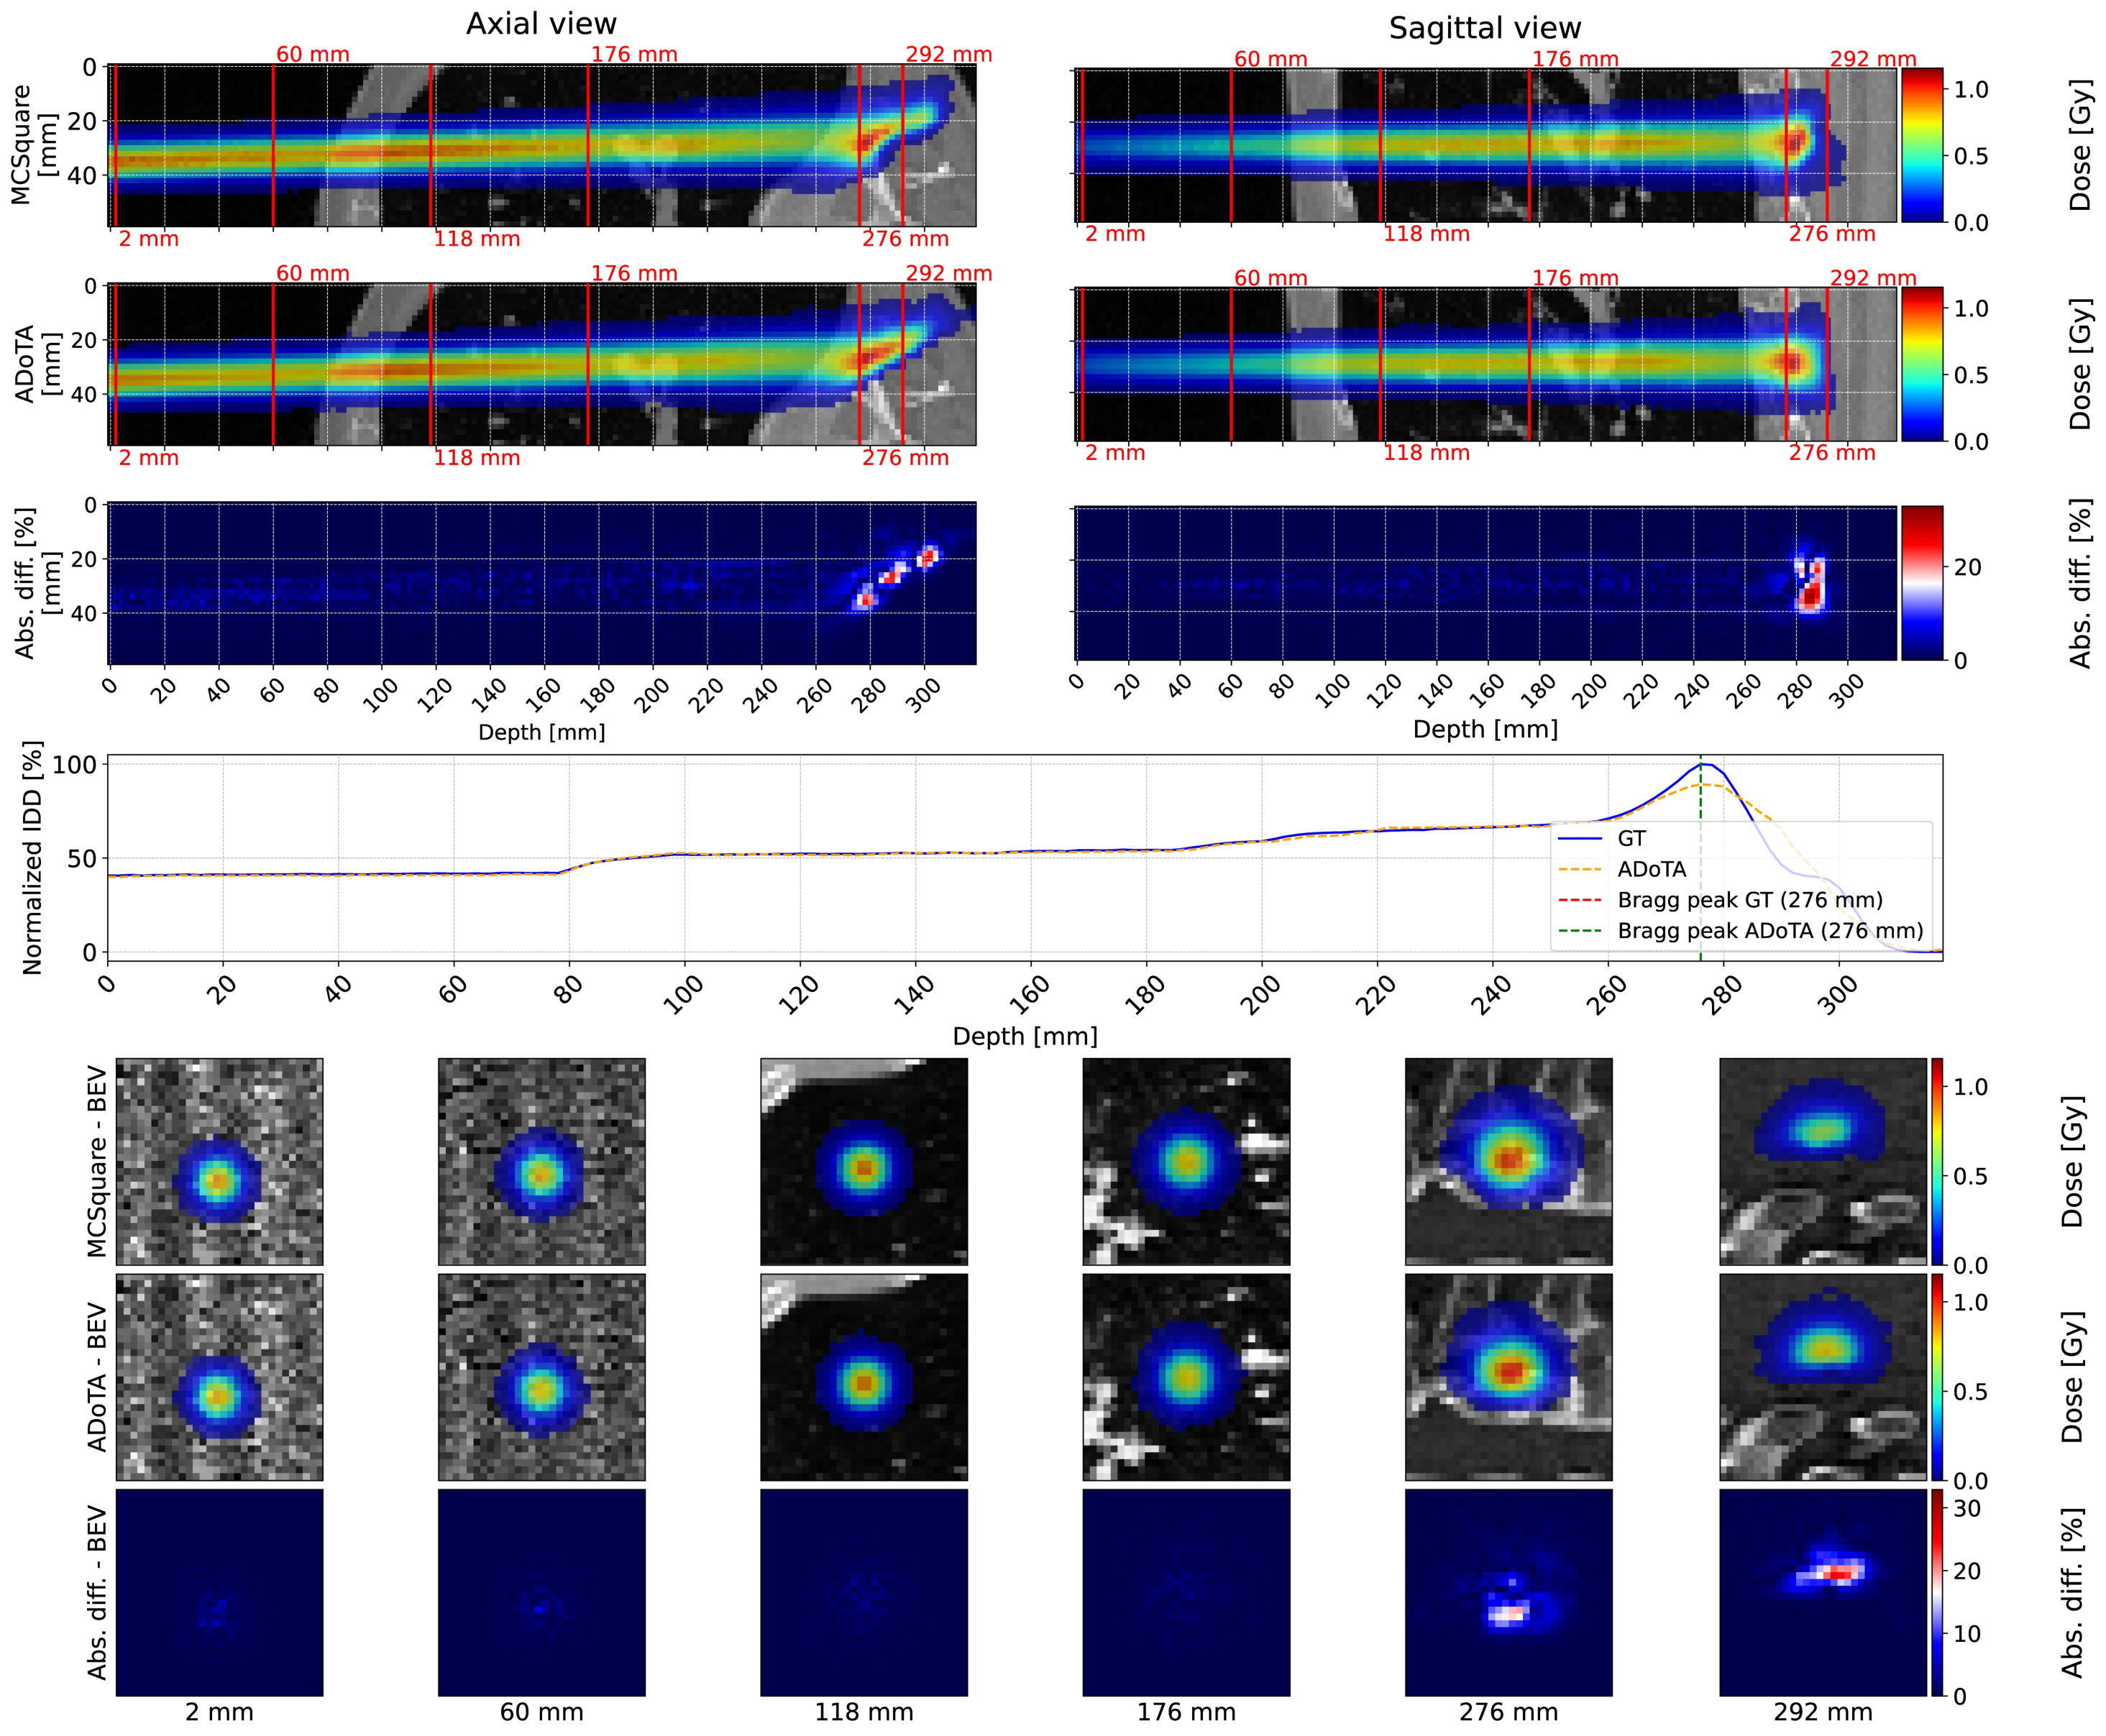
\includegraphics[width=0.92\linewidth,height=0.72\textheight,keepaspectratio]{figures/lung_mean.pdf}
  \end{center}

  \vspace{-2pt}
  {\scriptsize
  \begin{itemize}\setlength{\itemsep}{1pt}
    \item Axial (top) and sagittal (bottom) slices through the
          \textbf{mean predicted dose} across lung test beamlets.
    \item The model captures the lateral spread and Bragg peak
          position well, even in the presence of lung tissue
          heterogeneity.
    \item Largest deviations are visible near \textbf{tissue
          boundaries} (rib--lung, mediastinum), consistent with
          the lower GPR of $98.33\%$ for lung.
  \end{itemize}
  }
\end{frame}

\begin{frame}{Visual Results: Abdominal/Pelvic Test Cases (Axial \& Sagittal)}
  \vspace{-4pt}
  \begin{center}
    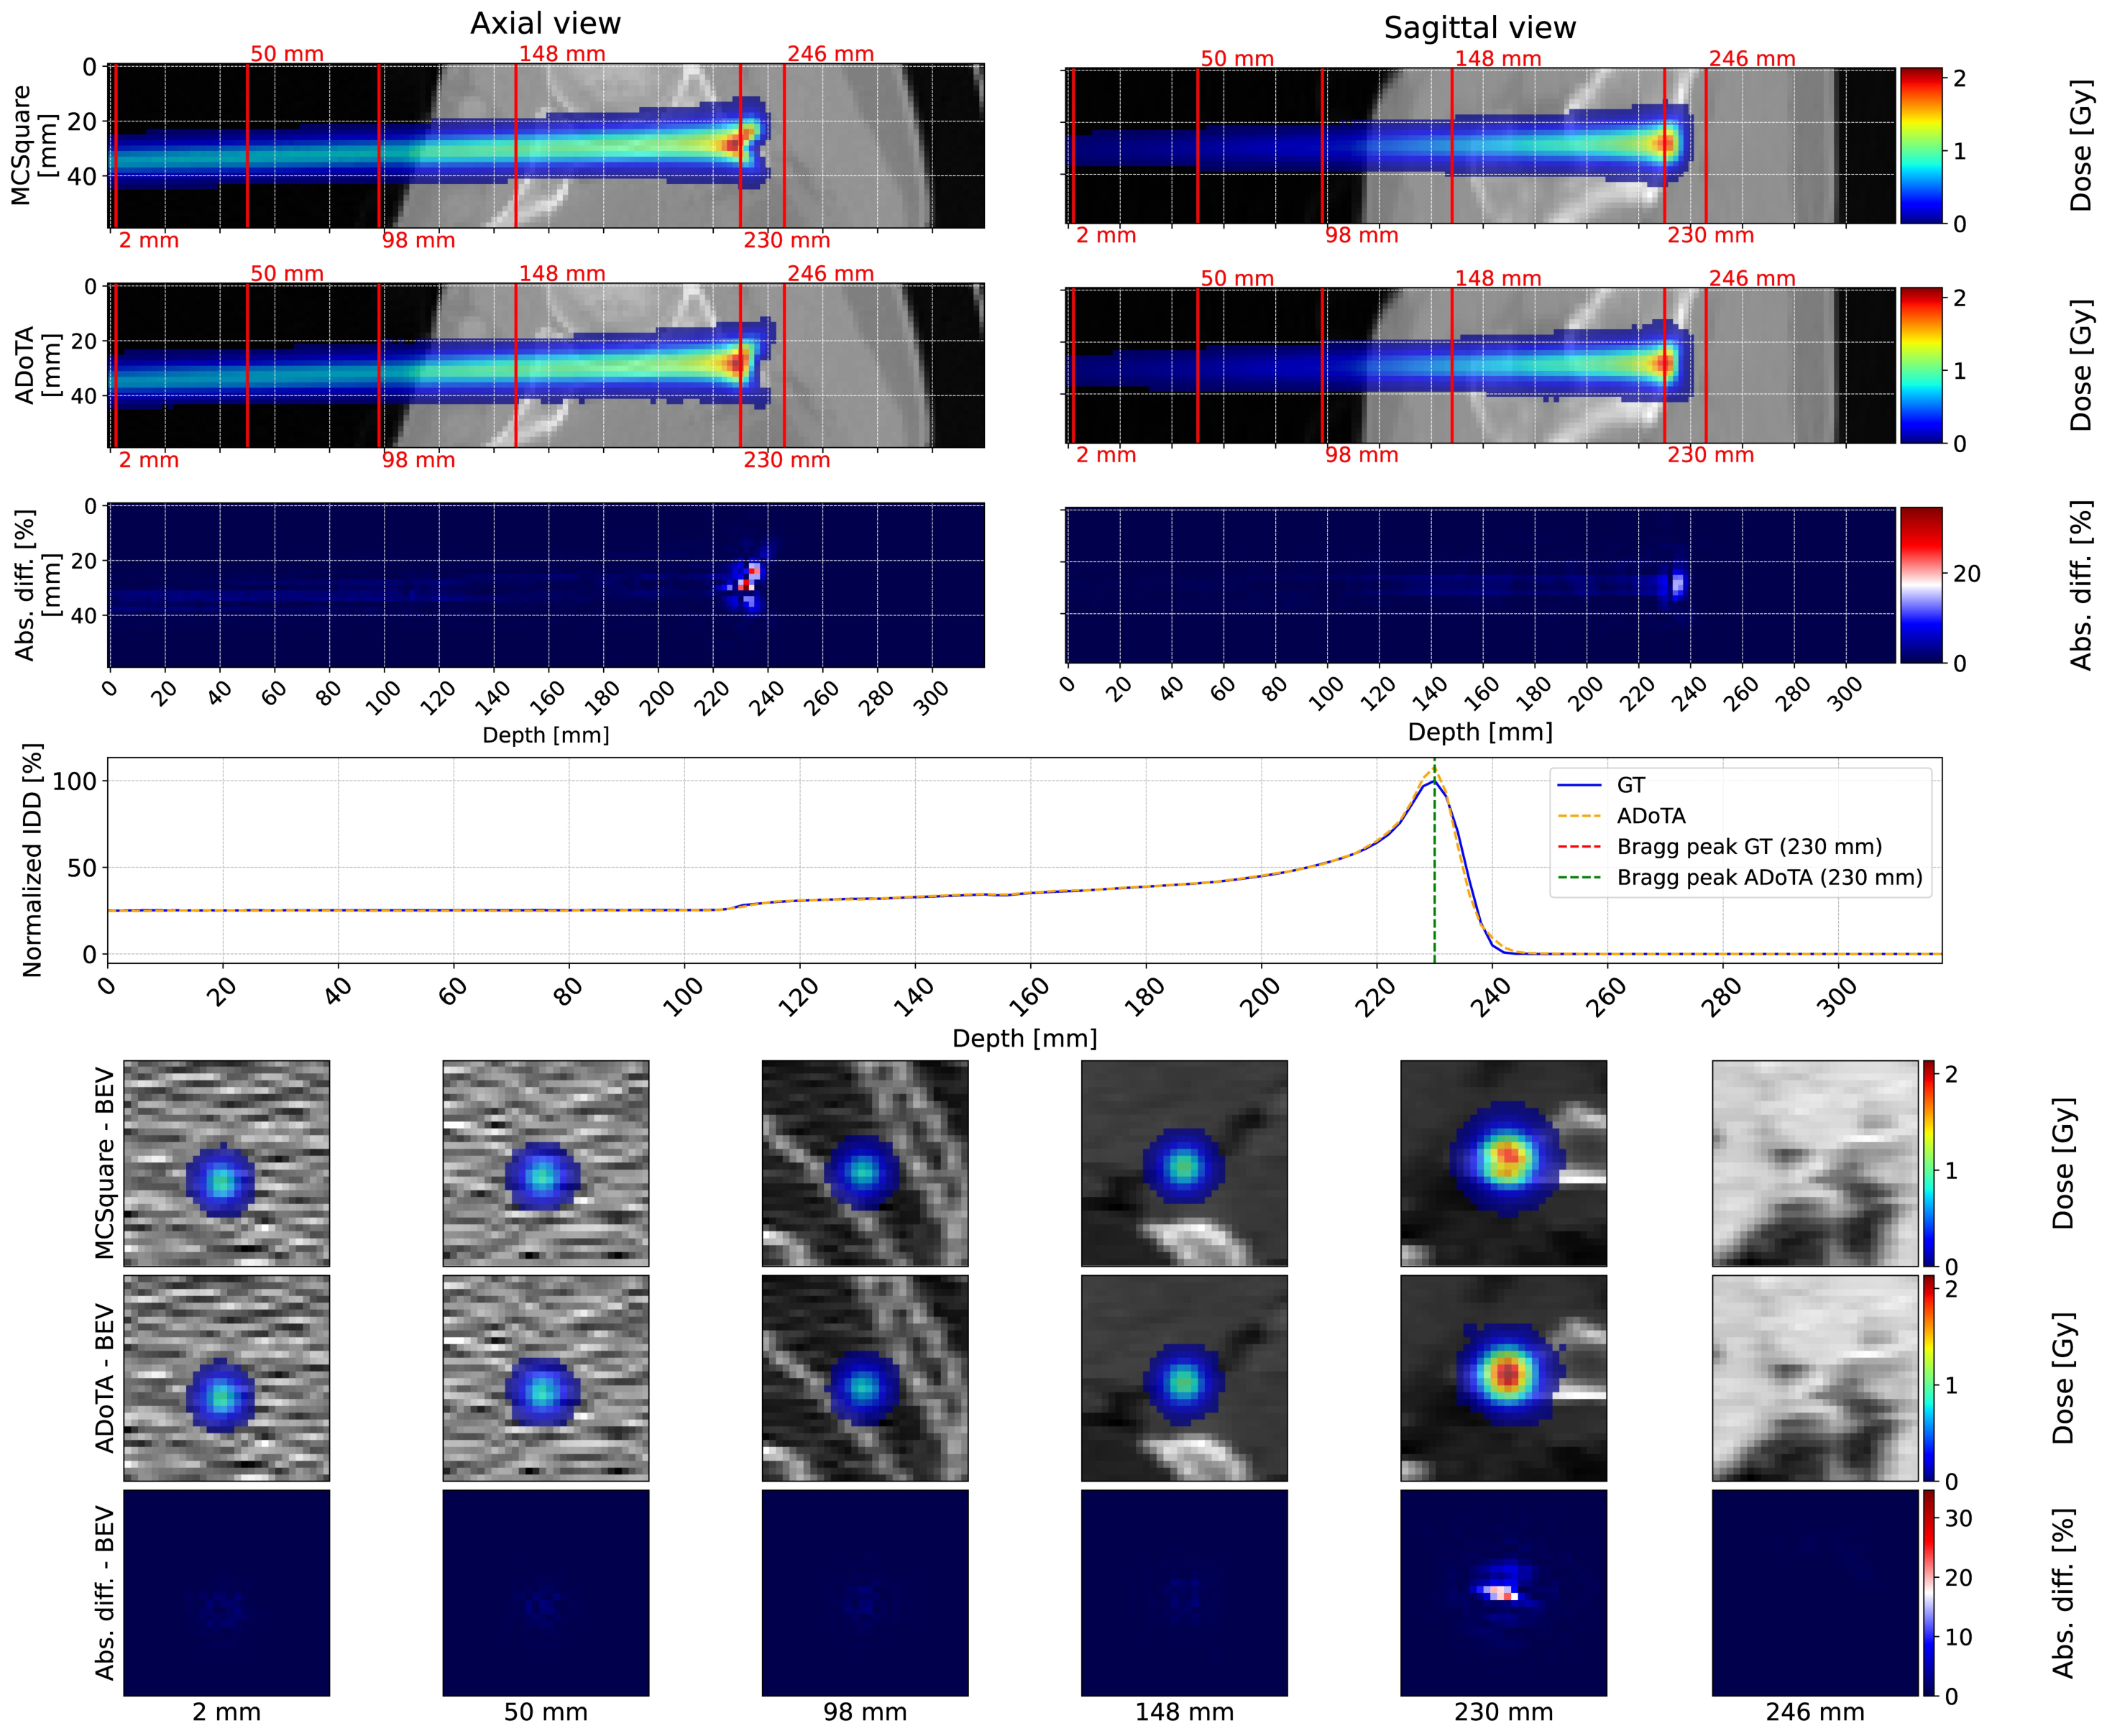
\includegraphics[width=0.92\linewidth,height=0.72\textheight,keepaspectratio]{figures/pelvic_abdominal_mean.pdf}
  \end{center}

  \vspace{-2pt}
  {\scriptsize
  \begin{itemize}\setlength{\itemsep}{1pt}
    \item Same representation for the abdominal/pelvic cohort —
          axial and sagittal views.
    \item Dose distributions are visually nearly
          \textbf{indistinguishable} from the Monte Carlo reference,
          matching the high GPR of $99.63\%$.
    \item More homogeneous tissue composition in this region leads
          to smoother dose gradients and smaller prediction errors.
  \end{itemize}
  }
\end{frame}

\begin{frame}{Test Set Statistics: Distribution of Metrics (3\,500 Beamlets)}
  \vspace{-4pt}
  \begin{center}
    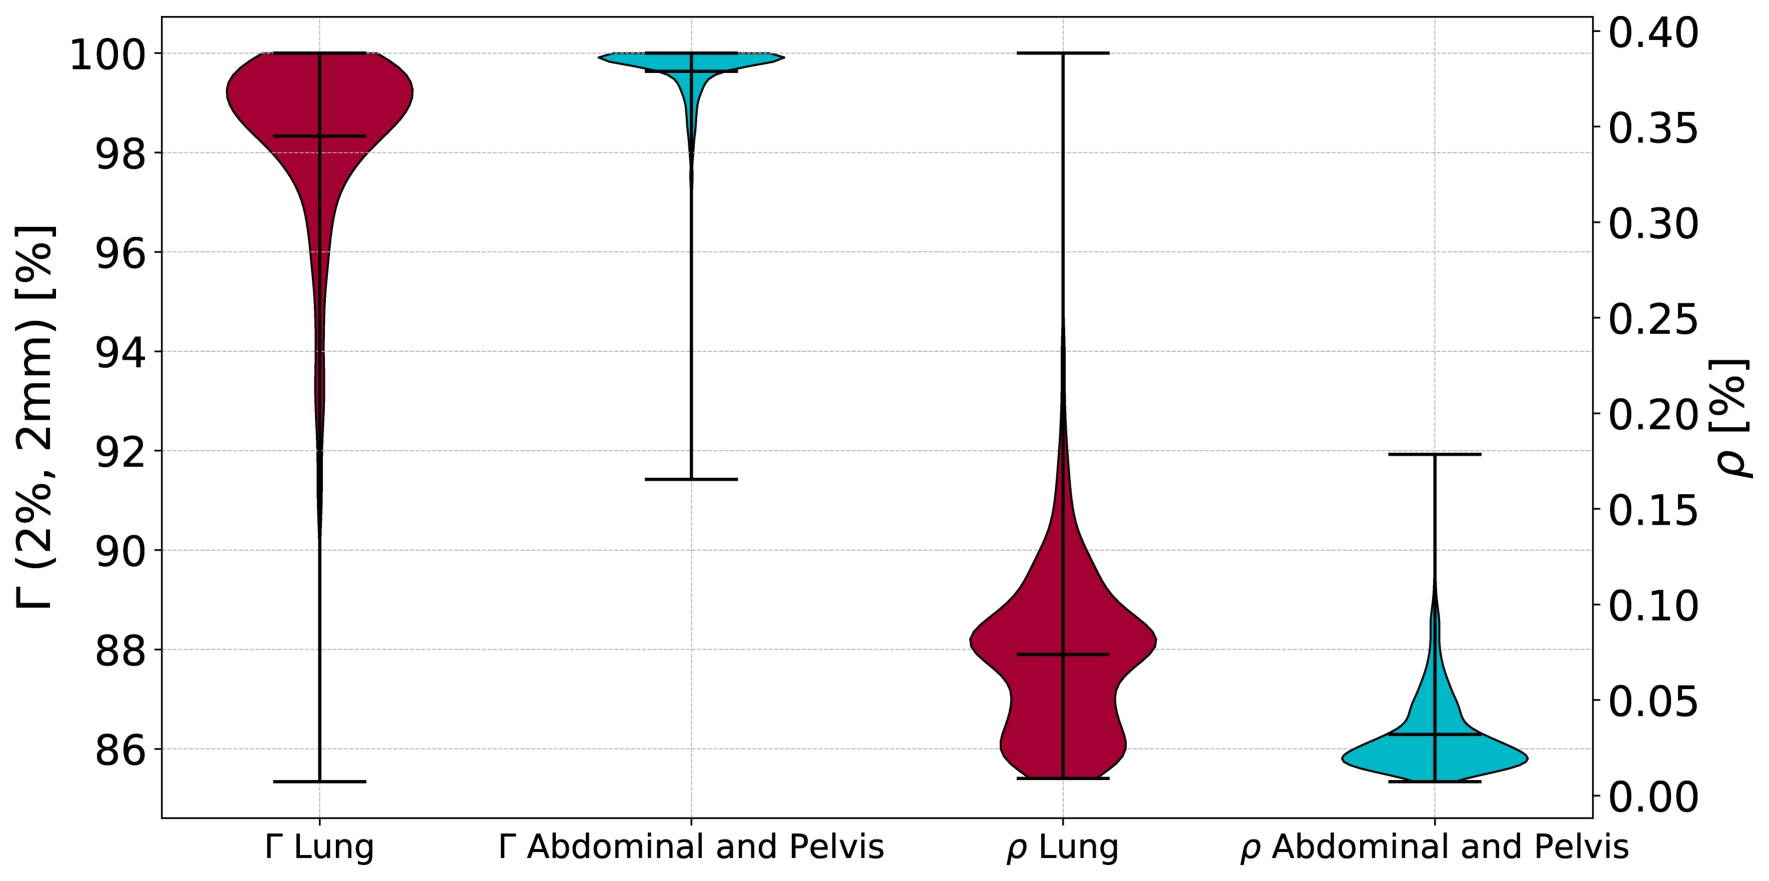
\includegraphics[width=0.88\linewidth,height=0.68\textheight,keepaspectratio]{figures/violin_histogram_testset_3500_combined.pdf}
  \end{center}

  \vspace{-2pt}
  {\scriptsize
  \begin{itemize}\setlength{\itemsep}{1pt}
    \item Violin plots and histograms of GPR, RDE, and RMSE across
          the full 3\,500-beamlet test set.
    \item The distributions are \textbf{tightly concentrated} near
          ideal values — the vast majority of beamlets achieve
          GPR~$>$~97\% with very low RDE and RMSE.
    \item The \textbf{long tails} correspond to challenging cases
          (tissue interfaces, high-energy deep beamlets) — precisely
          the samples that motivate active learning.
  \end{itemize}
  }
\end{frame}

\begin{frame}{Full Treatment Plan Validation}
  \begin{table}
    \centering\small
    \begin{tabular}{lccc}
      \toprule
      \textbf{Plan} & \textbf{Beamlets} & \textbf{Beams} &
        $\boldsymbol{\Gamma}$\textbf{(2\%/2mm, 10\%) [\%]} \\
      \midrule
      Prostate 1 & 1\,477 & 1 & 99.19 \\
      Prostate 2 & 4\,069 & 2 & 98.89 \\
      Prostate 3 & 2\,955 & 2 & 98.67 \\
      Prostate 4 & 3\,189 & 2 & 98.95 \\
      \midrule
      Lung 1     & 13\,392 & 1 & 97.56 \\
      Lung 2     & 82      & 2 & 98.54 \\
      Lung 3     & 1\,323  & 1 & 98.87 \\
      Lung 4     & 2\,899  & 1 & 98.78 \\
      \bottomrule
    \end{tabular}
  \end{table}

  \vspace{4pt}
  \begin{itemize}
    \item 8 treatment plans (4 prostate, 4 lung) computed end to end
          with ADoTA.
    \item All plans achieve $>$ \SI{97.5}{\percent} GPR.
    \item Prostate mean: \SI{98.93}{\percent}, Lung mean:
          \SI{98.44}{\percent}.
    \item Errors are \textbf{systematic} (not stochastic like MC noise)
          — neighbouring beamlets share similar anatomy, so local errors
          accumulate rather than cancel.
  \end{itemize}
\end{frame}

\begin{frame}{Runtime: The Speed Advantage}
  \begin{columns}[T]
    \begin{column}{0.48\textwidth}
      \textbf{Inference time per beamlet:}
      \begin{table}
        \centering\small
        \begin{tabular}{lc}
          \toprule
          \textbf{Model} & \textbf{Time/beamlet} \\
          \midrule
          Monte Carlo       & \SI{43.6}{s}  \\
          PBA               & \SI{728}{ms}  \\
          DoTA              & \SI{5.0}{ms}  \\
          \textbf{ADoTA}    & \textbf{\SI{1.75}{ms}} \\
          \bottomrule
        \end{tabular}
      \end{table}

      \vspace{4pt}
      {\small ADoTA is $\sim$25\,000$\times$ faster than MC and
       $\sim$3$\times$ faster than DoTA (batch size 56).}
    \end{column}
    \begin{column}{0.48\textwidth}
      \textbf{End-to-end pipeline comparison:}

      \vspace{4pt}
      \begin{itemize}\setlength{\itemsep}{4pt}
        \item \textbf{Prior methods}: reinterpolate CT per beamlet\\
              $\Rightarrow$ \SI{1.3}{s} preprocessing +
              \SI{5}{ms} inference\\
              = \SI{1.3}{s}/beamlet.
        \item \textbf{ADoTA}: reinterpolate per gantry angle,
              compute $\Phi$ analytically\\
              $\Rightarrow$ \SI{0.2}{s}/beamlet total.
        \item \textbf{Speedup}: $\sim$6.5$\times$ end-to-end
              reduction vs.\ DoTA pipeline.
      \end{itemize}

      \vspace{6pt}
      \begin{block}{Outlook}
        Porting ray-tracing and $\Phi$ construction to GPU
        $\rightarrow$ sub-second total for thousands of beamlets.
      \end{block}
    \end{column}
  \end{columns}
\end{frame}

% ════════════════════════════════════════════════════════════════
\section{Limitations and Open Challenges}
% ════════════════════════════════════════════════════════════════

\begin{frame}{Known Limitations}
  \begin{columns}[T]
    \begin{column}{0.48\textwidth}
      \textbf{1.\ Tissue interface degradation}
      \begin{itemize}\setlength{\itemsep}{3pt}
        \item Beamlets whose Bragg peak lies at a tissue interface
              (bone to soft tissue, air to tissue) are \textbf{harder to
              predict}.
        \item GPR gap: $\sim$0.7\,pp between interface and homogeneous
              beamlets.
        \item 24 to 40\% of training beamlets are affected (depending
              on the neighbourhood radius).
        \item This gap is \textbf{robust} across thresholds
              $\tau \in [50, 400]$\,HU and radii $r \in \{5, 10\}$\,mm.
      \end{itemize}
    \end{column}
    \begin{column}{0.48\textwidth}
      \textbf{2.\ Depth dependent performance}
      \begin{itemize}\setlength{\itemsep}{3pt}
        \item GPR degrades in the distal 25\% of the dose volume,
              coinciding with the Bragg peak region.
        \item Caused by (a) data sparsity at large penetration depths
              and (b) steep gradients + range straggling.
      \end{itemize}

      \vspace{6pt}
      \textbf{3.\ Systematic plan level errors}
      \begin{itemize}\setlength{\itemsep}{3pt}
        \item Neighbouring beamlets traverse similar anatomy
              $\Rightarrow$ errors accumulate rather than cancel.
        \item Most pronounced in lung (heterogeneous media).
      \end{itemize}
    \end{column}
  \end{columns}
\end{frame}

\begin{frame}{The Tissue Interface Problem: A Concrete Example}
  \vspace{-4pt}
  \begin{columns}[T]
    \begin{column}{0.55\textwidth}
      \begin{center}
        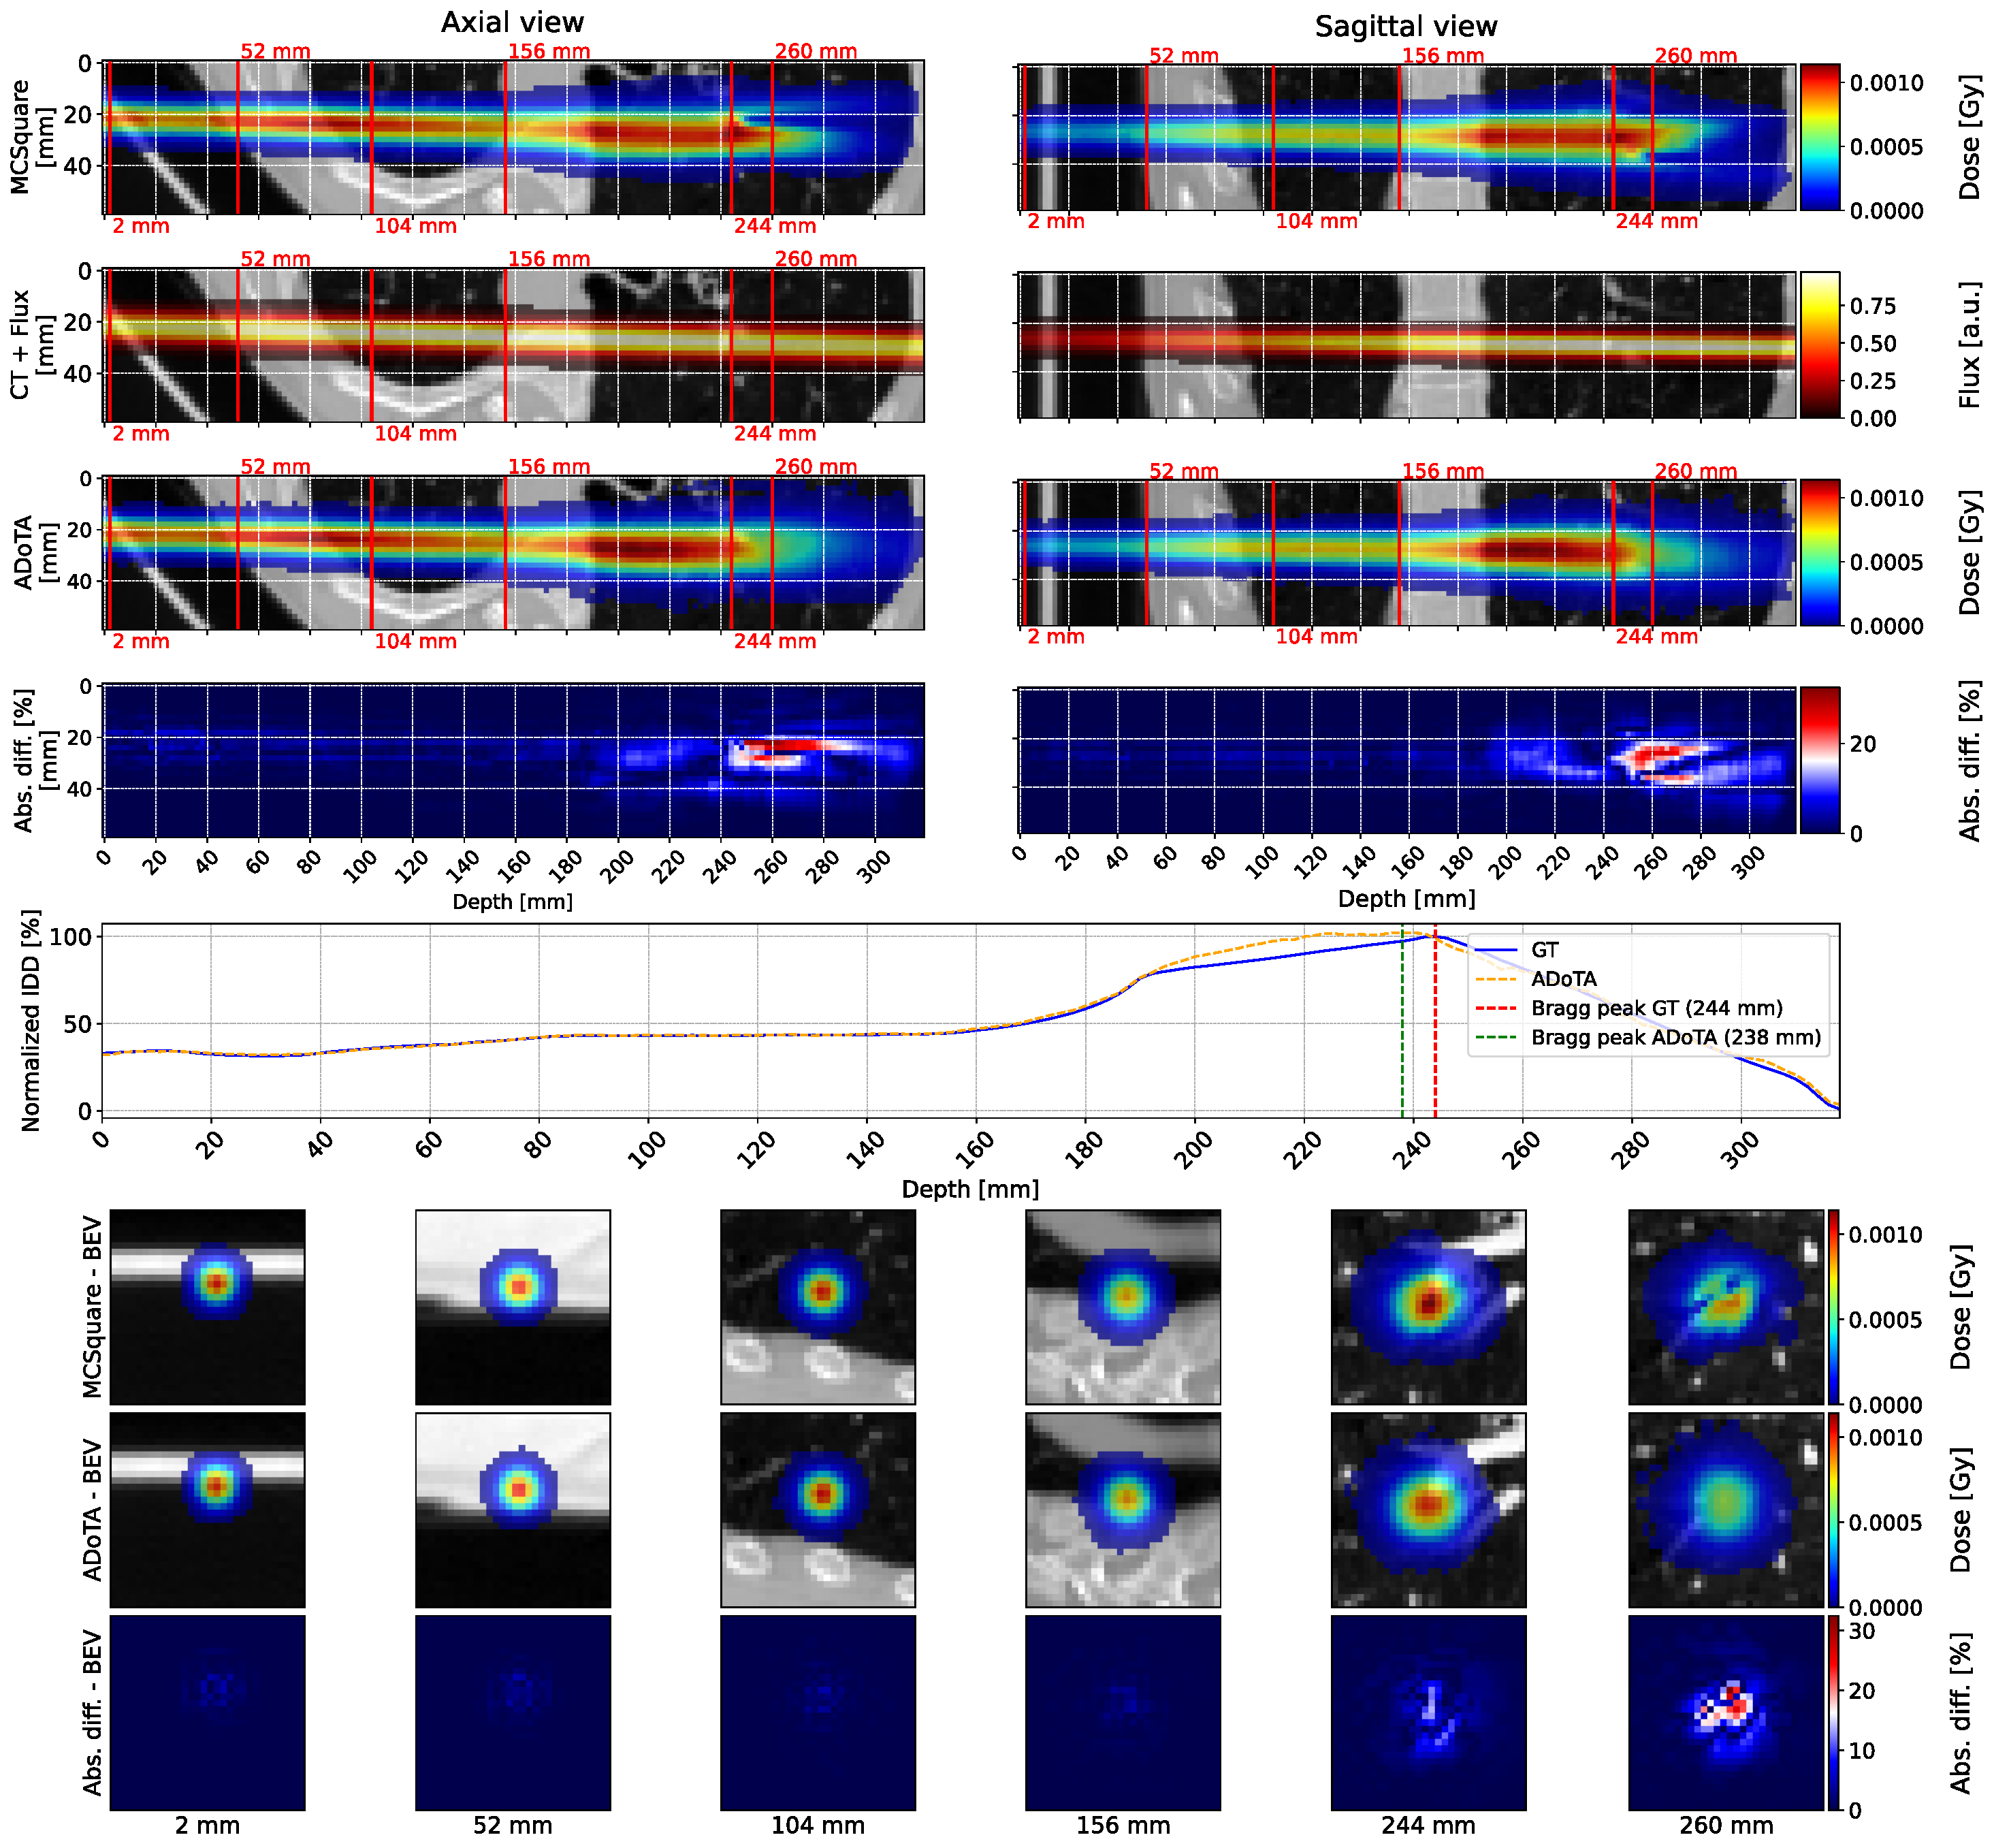
\includegraphics[width=\linewidth,height=0.78\textheight,keepaspectratio]{figures/Interface_Worst_005_E123.53MeV.pdf}
      \end{center}
    \end{column}
    \begin{column}{0.42\textwidth}
      {\small\textbf{What are we looking at?}}

      \vspace{3pt}
      {\scriptsize
      A beamlet at $E = 123.5$\,MeV whose Bragg peak falls
      exactly at a tissue interface. The top row shows axial and
      sagittal views; the bottom row shows the depth dose profile
      (IDD) and the local gamma analysis.
      }

      \vspace{6pt}
      {\small\textbf{What goes wrong?}}

      \vspace{3pt}
      {\scriptsize
      \begin{itemize}\setlength{\itemsep}{2pt}
        \item The Bragg peak position and amplitude are
              \textbf{mispredicted} because the abrupt density
              change at the interface alters the proton range
              in a way the model has not learned well enough.
        \item The lateral dose spread is also affected: density
              discontinuities scatter protons differently than
              homogeneous tissue.
        \item These are the \textbf{worst performing beamlets} in
              the test set and they share a common trait: tissue
              heterogeneity around the Bragg peak.
      \end{itemize}
      }

      \vspace{4pt}
      {\scriptsize\color{tudelft}
       $\Rightarrow$ This is exactly why we need a
       \textbf{targeted} training strategy that focuses on these
       challenging regions.}
    \end{column}
  \end{columns}
\end{frame}

\begin{frame}{Why Tissue Interfaces Matter}
  \begin{columns}[T]
    \begin{column}{0.55\textwidth}
      \textbf{Our analysis} (69\,295 pelvis beamlets):

      \vspace{4pt}
      \begin{table}
        \centering\small
        \begin{tabular}{lcc}
          \toprule
          \textbf{Group} & \textbf{GPR [\%]} & \textbf{MAPE [\%]} \\
          \midrule
          Homogeneous  & $99.11 \pm 1.23$ & $5.11 \pm 1.63$ \\
          Interface    & $98.41 \pm 1.68$ & $6.12 \pm 2.09$ \\
          \midrule
          Gap          & 0.70\,pp         & 1.01\,pp \\
          \bottomrule
        \end{tabular}
      \end{table}

      \vspace{4pt}
      \begin{itemize}\setlength{\itemsep}{2pt}
        \item Classification: $\sigma_{\text{HU}} > \SI{200}{HU}$
              in a sphere of radius $r = \SI{10}{mm}$ around the
              estimated Bragg peak.
        \item The gap persists across all four metrics (GPR, MAPE,
              RDE, RMSE) and across threshold sweeps
              $\tau \in [50, 400]$\,HU.
      \end{itemize}
    \end{column}
    \begin{column}{0.42\textwidth}
      \textbf{Implication:}

      \vspace{4pt}
      The model struggles where it matters most — at tissue
      boundaries where dose gradients are clinically critical.

      \vspace{8pt}
      \textbf{Root cause:}
      \begin{itemize}\setlength{\itemsep}{3pt}
        \item Density discontinuities create complex scattering
              and range effects.
        \item The training set does not distinguish ``easy''
              from ``hard'' samples — uniform sampling treats
              all beamlets equally.
      \end{itemize}

      \vspace{8pt}
      {\small\color{tudelft} $\Rightarrow$ This motivates a
       \textbf{smarter} training strategy.}
    \end{column}
  \end{columns}
\end{frame}

% ════════════════════════════════════════════════════════════════
\section{The Case for Active Learning}
% ════════════════════════════════════════════════════════════════

\begin{frame}{What Is Active Learning?}
  \begin{columns}[T]
    \begin{column}{0.55\textwidth}
      \textbf{Standard training:}
      \begin{enumerate}
        \item Generate a large labelled dataset (MC simulations).
        \item Train on all samples uniformly.
        \item Hope the model generalises.
      \end{enumerate}

      \vspace{6pt}
      \textbf{Active learning:}
      \begin{enumerate}
        \item Start with a small labelled set.
        \item Train the model.
        \item \textbf{Query} the most informative unlabelled samples.
        \item Label only those (run MC simulation).
        \item Retrain and repeat.
      \end{enumerate}

      \vspace{4pt}
      {\small The model \emph{chooses} what to learn from, reducing
       the total number of expensive MC simulations needed.}
    \end{column}
    \begin{column}{0.42\textwidth}
      \begin{center}
        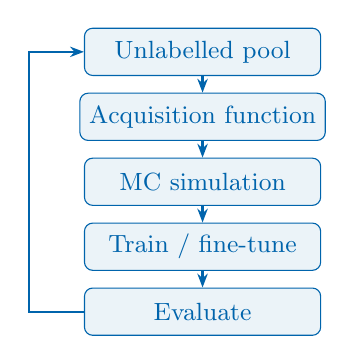
\begin{tikzpicture}[
          box/.style={draw=tudelft, rounded corners=3pt,
                      minimum width=3cm, minimum height=0.6cm,
                      font=\small, text=tudelft, fill=tudelft!8},
          arr/.style={-{Stealth[length=5pt]}, thick, tudelft}
        ]
          \node[box] (pool) {Unlabelled pool};
          \node[box, below=6pt of pool] (acq) {Acquisition function};
          \node[box, below=6pt of acq] (label) {MC simulation};
          \node[box, below=6pt of label] (train) {Train / fine-tune};
          \node[box, below=6pt of train] (eval) {Evaluate};
          \draw[arr] (pool) -- (acq);
          \draw[arr] (acq) -- (label);
          \draw[arr] (label) -- (train);
          \draw[arr] (train) -- (eval);
          \draw[arr] (eval.west) -- ++(-0.7,0)
                     |- (pool.west);
        \end{tikzpicture}
      \end{center}
    \end{column}
  \end{columns}
\end{frame}

\begin{frame}{Why Active Learning for ADoTA?}
  \begin{columns}[T]
    \begin{column}{0.48\textwidth}
      \textbf{The labelling bottleneck:}
      \begin{itemize}\setlength{\itemsep}{4pt}
        \item Each training label = one MC simulation
              ($10^7$ protons, \SI{43.6}{s}).
        \item Current training set: 70\,285 beamlets
              $\Rightarrow$ $\sim$850 CPU-hours of MC time.
        \item Expanding to new anatomies, energies, or angles
              multiplies this cost.
      \end{itemize}

      \vspace{6pt}
      \textbf{The performance gap is not uniform:}
      \begin{itemize}\setlength{\itemsep}{4pt}
        \item The model is already excellent on homogeneous regions
              (GPR $\approx$ 99.1\%).
        \item The deficit is concentrated at tissue interfaces.
        \item Uniform data collection wastes budget on ``easy''
              samples the model already handles well.
      \end{itemize}
    \end{column}
    \begin{column}{0.48\textwidth}
      \textbf{Physics-informed acquisition:}

      \vspace{4pt}
      Our tissue interface analysis provides \textbf{cheap,
      precomputable proxies} for prediction difficulty:

      \vspace{4pt}
      \begin{itemize}\setlength{\itemsep}{4pt}
        \item $\sigma_{\text{HU}}$: CT density standard deviation
              around the Bragg peak.
        \item TV: total variation of HU values in the neighbourhood.
        \item These correlate strongly with GPR degradation
              and can be computed in milliseconds from CT alone
              — no model inference needed.
      \end{itemize}

      \vspace{6pt}
      \begin{block}{Proposed strategy}
        Use $\sigma_{\text{HU}}$ and TV as \textbf{acquisition
        functions} to preferentially select interface-heavy beamlets
        for MC simulation and targeted fine-tuning.
      \end{block}
    \end{column}
  \end{columns}
\end{frame}

\begin{frame}{Expected Benefits}
  \begin{enumerate}\setlength{\itemsep}{6pt}
    \item \textbf{Reduced MC simulation budget} — focus expensive
          labels on the beamlets where the model needs them most,
          rather than uniformly sampling the anatomy.

    \item \textbf{Faster gap closure} — targeted fine-tuning on
          interface-heavy batches should close the GPR gap more
          efficiently than retraining on the full dataset.

    \item \textbf{Principled extension to new sites} — when deploying
          ADoTA to a new anatomy (e.g.\ head and neck), active
          learning identifies the hardest regions automatically,
          minimising the amount of new MC data required.

    \item \textbf{Quantitative stopping criterion} — monitor the
          interface vs.\ homogeneous GPR gap across active learning
          iterations; stop when the gap falls below a clinical
          threshold.

    \item \textbf{Better uncertainty quantification} — the acquisition
          function naturally flags beamlets that should be treated with
          caution in clinical QA workflows.
  \end{enumerate}
\end{frame}

% ════════════════════════════════════════════════════════════════
\section{Summary \& Next Steps}
% ════════════════════════════════════════════════════════════════

\begin{frame}{Summary}
  \begin{enumerate}\setlength{\itemsep}{4pt}
    \item \textbf{ADoTA} is a deep learning proton dose engine that
          eliminates per-beamlet CT reinterpolation by conditioning
          on an analytical beamlet shape projection $\Phi$.
    \item It achieves \textbf{MC-level accuracy}
          (GPR $> 98\%$ on treatment plans) at
          \textbf{\SI{1.75}{ms}/beamlet} — 25\,000$\times$ faster
          than MC.
    \item \textbf{Tissue interfaces} remain the dominant source of
          prediction error, with a robust $\sim$0.7\,pp GPR gap
          that persists across all tested radii and thresholds.
    \item This systematic performance gap motivates
          \textbf{active learning}: using physics-informed
          heterogeneity metrics ($\sigma_{\text{HU}}$, TV) as
          acquisition functions to guide targeted data collection
          and fine-tuning.
  \end{enumerate}
\end{frame}

\begin{frame}{Next Steps}
  \begin{enumerate}\setlength{\itemsep}{5pt}
    \item \textbf{Design acquisition function} — combine
          $\sigma_{\text{HU}}$, TV, and CV into a composite score
          for selecting the most informative beamlets from the
          unlabelled pool.
    \item \textbf{Active learning loop} — implement the
          select $\rightarrow$ simulate $\rightarrow$ fine-tune
          $\rightarrow$ evaluate cycle and measure gap closure rate.
    \item \textbf{Multi-radius analysis} — compute heterogeneity
          at $r \in \{5, 10, 15, 20, 30\}$\,mm to determine the
          optimal neighbourhood for the acquisition function.
    \item \textbf{Energy-stratified analysis} — investigate whether
          the interface effect is stronger at specific beam energies.
    \item \textbf{New anatomical sites} — extend the analysis to
          lung data, where tissue interfaces are more prevalent.
  \end{enumerate}
\end{frame}

% ── Closing ─────────────────────────────────────────────────
\begin{frame}[plain]
  \begin{center}
    \vspace{2cm}
    {\Huge\color{tudelft} Thank you}\\[12pt]
    {\large Questions \& discussion}\\[20pt]
    {\small Mikołaj Stryja \textbar{} \texttt{m.a.stryja@tudelft.nl}}
  \end{center}
\end{frame}

\end{document}
